\scanpage{79}
% @0 upper right
\mspage{- 25 -}
% @1–2 continuation bracket
\noindent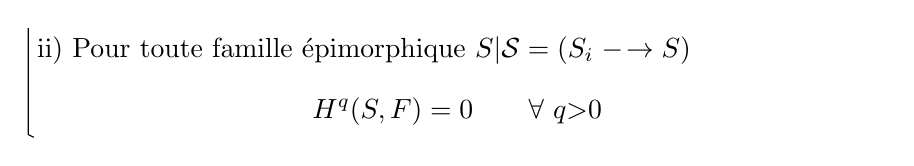
\begin{tikzpicture}
\node[inner sep=3pt] (ii) {\begin{minipage}{.88\linewidth}
ii) Pour toute famille épimorphique $\handwritten{\unsure{\mathscr S|\mathcal S}}=(S_i\mathrel{\relbar\joinrel\handwritten{\rightarrow}}S)$
\[
 H^q(\handwritten{\mathscr S},F)=0\qquad \handwritten{\forall}\ q\handwritten{>}0
\]
\end{minipage}};
\handwritten{\draw (ii.north west) -- (ii.south west) -- ++(2pt,-1pt);}
\end{tikzpicture}

% @3–4 forward implication
\uline{Preuve} : (i) $\handwritten{\Longrightarrow}$ (ii). Se déduit immédiatement de la suite exacte de la proposition 1.5

% @5–6 converse
(ii) $\handwritten{\Longrightarrow}$ (i). Soit $S$ un objet de $E$. Il existe une sous-catégorie pleine $C$ de $E$ qui possède les propriétés suivantes :

% @7–8 clause a
a) L'ensemble des objets de $C$ peut être indexé par un élément de l'univers et est une famille de générateurs de $E$.

% @9 clause b
b) Les produits fibrés sont représentables dans $C$.

% @10 clause c
\tikz[baseline=(cc.base)]{\node[inner sep=1pt] (cc) {c)};\handwritten{\draw (cc.north east) ++(-1pt,3pt) -- ++(0,-3pt) .. controls +(-16pt,2pt) and +(-14pt,-5pt) .. (cc.south east) -- ++(0,-2pt);}} L'objet $S$ est un objet de $C$.

% @11–14 topology
Munissons alors $C$ de la topologie induite par $E$. La catégorie des faisceaux d'ensembles sur $C$ est équivalente à $E$ (3.5.4.III). Le faisceau $F$ induit alors sur $C$ un faisceau $C$-acyclique ((3.1) et (1.6)) par suite :
% @15 vanishing
\[
 H^q(S,F)=0\qquad\handwritten{\forall}\ q\handwritten{>}0
\]
% @16 closing
\hfill c.q.f.d.

% @17–21 definition bracket
\noindent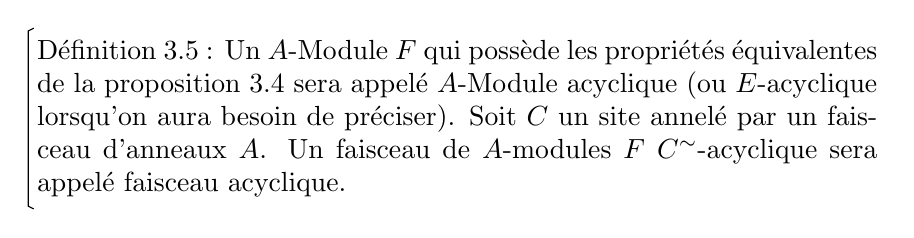
\begin{tikzpicture}
\node[inner sep=3pt] (defn) {\begin{minipage}{.88\linewidth}
\uline{Définition 3.5} : Un $A$-Module $F$ qui possède les propriétés équivalentes de la proposition 3.4 sera appelé $A$-Module \uline{acyclique} (ou $E$-acyclique lorsqu'on aura besoin de préciser). Soit $C$ un site annelé par un faisceau d'anneaux $A$. Un faisceau de $A$-modules $F$ $C^{\handwritten{\sim}}$-acyclique sera appelé faisceau \uline{acyclique}.
\end{minipage}};
\handwritten{\draw (defn.north west) ++(2pt,1pt) -- (defn.north west) -- (defn.south west) -- ++(2pt,-1pt);}
\end{tikzpicture}
% @22 foot
\hfill \ldots/\ldots
% archive sheet number: 78

